\documentclass[11pt]{article}
%Gummi|063|=)
\usepackage{amsmath}
\usepackage[authoryear, round]{natbib}
\usepackage{graphicx}
\usepackage{caption}

\title{\textbf{Financial Econometric Models}}
\author{Johannes Degn}
\date{04.02.2014}
\begin{document}

\maketitle

\section{Univariate type-ARCH models}

\section{Multivariate type-ARCH models}
\subsection{}
\subsubsection{BEKK(1,1,1)}
i) \\
$$H_t = C'C + A'\varepsilon_{t-1}\varepsilon_{t-1}'A + B'H_{t-1}B$$
$
H_t = \begin{pmatrix}
c_1 & 0 \\
c_2 & c_3 \\
\end{pmatrix}
\begin{pmatrix}
c_1 & c_2 \\
0 & c_3 \\
\end{pmatrix}
+
\begin{pmatrix}
a_1 & 0 \\
0 & a_2 \\
\end{pmatrix}
\begin{pmatrix}
\varepsilon_{t-1, 1} \\
\varepsilon_{t-1, 2} \\
\end{pmatrix}
\begin{pmatrix}
\varepsilon_{t-1, 1} & \varepsilon_{t-1, 2} \\
\end{pmatrix}
\begin{pmatrix}
a_1 & 0 \\
0 & a_2 \\
\end{pmatrix}
+
\begin{pmatrix}
b_1 & 0 \\
0 & b_2 \\
\end{pmatrix}
\begin{pmatrix}
h_{t-1, 11} & h_{t-1, 12} \\
h_{t-1, 21} & h_{t-1, 22} \\
\end{pmatrix}
\begin{pmatrix}
b_1 & 0 \\
0 & b_2 \\
\end{pmatrix}
$
\\
\\
\noindent
\\
$
H_t = \begin{pmatrix}
c_1^2 & c_1c_2 \\
c_1c_2 & c_2^2+c_3^2 \\
\end{pmatrix}
+
\begin{pmatrix}
a_1^2\varepsilon_{t-1, 1}^2 & a_1a_2\varepsilon_{t-1, 1}\varepsilon_{t-1, 2} \\
a_1a_2\varepsilon_{t-1, 1}\varepsilon_{t-1, 2} & a_2^2\varepsilon_{t-1, 2} \\
\end{pmatrix}
+
\begin{pmatrix}
b_1^2h_{t-1, 11} & b_1b_2h_{t-1, 12} \\
b_1b_2h_{t-1, 21} & b_2^2h_{t-1, 22} \\
\end{pmatrix}
$
\\
\\
\noindent $h_{t, 11}$, $h_{t, 22}$ and $h_{t, 12}$ can be read from the respective addition above.
\\
\\
\noindent
ii)
positivity constraints are satisfied as the diagonal elements ($h_{t, 11}$ and $h_{t, 22}$) are bigger than or equal to 0. TODO: CHECK THIS WHAT IS ASKED! \\
\\
iii) 
\begin{figure}[hc]
\centering
\caption{Simulated series of a BEKK(1,1,1)}
\caption*{parameters: $A = \begin{pmatrix} 
0.5 & 0 \\
0 & 0.5 \\
\end{pmatrix}$, $B = \begin{pmatrix} 
0.5 & 0 \\
0 & 0.5 \\
\end{pmatrix}$, $C = \begin{pmatrix} 
1 & 1 \\
0 & 1 \\
\end{pmatrix}$}
\label{correlogram1}
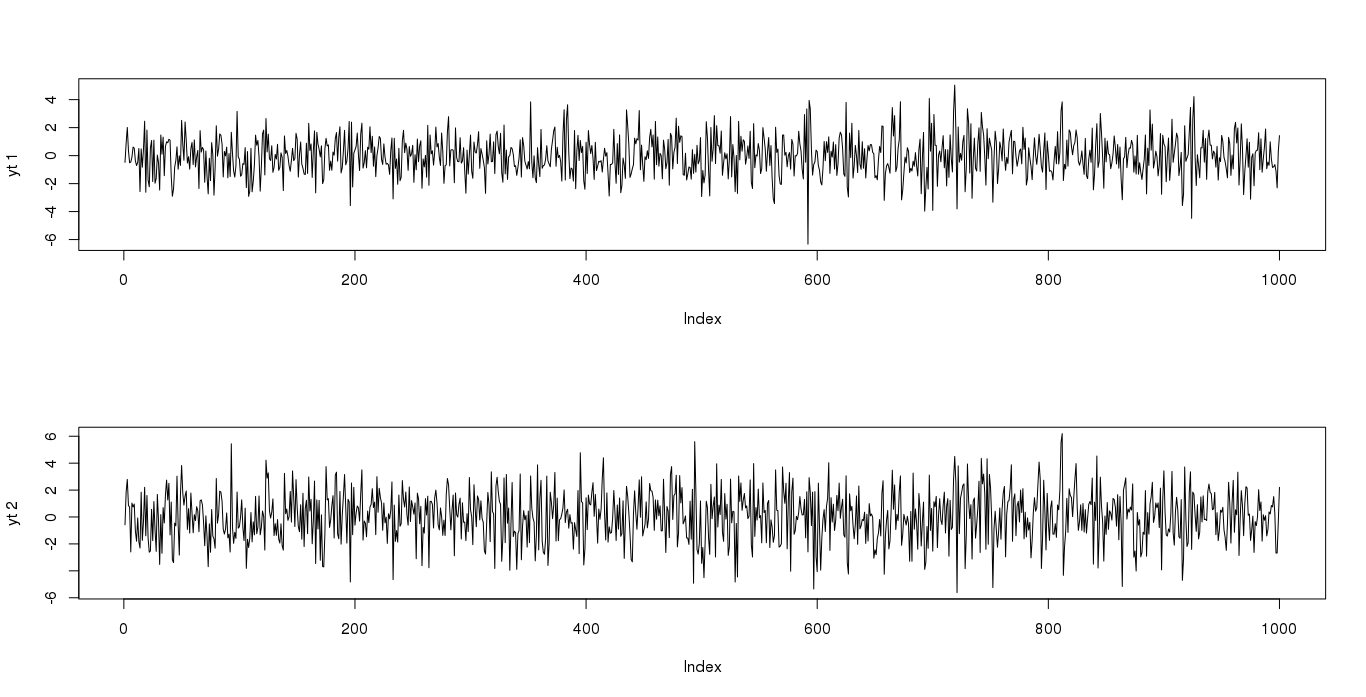
\includegraphics[width=160mm]{graphs/problem2_simulated_series.png}

\end{figure}

\bibliographystyle{plainnat}
\bibliography{/home/joi/workspace/latex/citations}
\end{document}
